\chapter{Proposta de Ferramenta}

Nesta seção, será apresentada uma ferramenta cujo objetivo é automatizar a geração de questões, com o objetivo de tornar mais fácil a construção e geração de questões. A ferramenta baseia-se em um modelo de separação entre duas entidades principais : (i) um JSON de template, responsável por definir a estrutura geral das questões; e (ii) um JSON de questões, que instancia as variações específicas de cada problema. O sistema foi planejado para permitir que os professores sejam responsáveis pela elaboração e manutenção dos templates. Por outro l ado os usuários estudantes interagem apenas com as questões geradas a partir desses templates.

\section{JSON de Templates}

O primeiro componente é o JSON de Template, ilustrado na Figura \ref{fig:json-de-templates}, no qual o enunciado geral (\textit{stem}) descreve a estrutura padrão que será aplicada em todas as questões derivadas. Nele, é definido as partes fixas do enunciado e a forma como os elementos variáveis serão combinados para formar a pergunta final. Em seguida, cada categoria de variáveis contém uma lista de opções textuais ou numéricas que podem assumir diferentes valores de acordo com a necessidade, permitindo a criação de múltiplas versões de um mesmo problema.


\begin{figure}[ht]
	\centering
	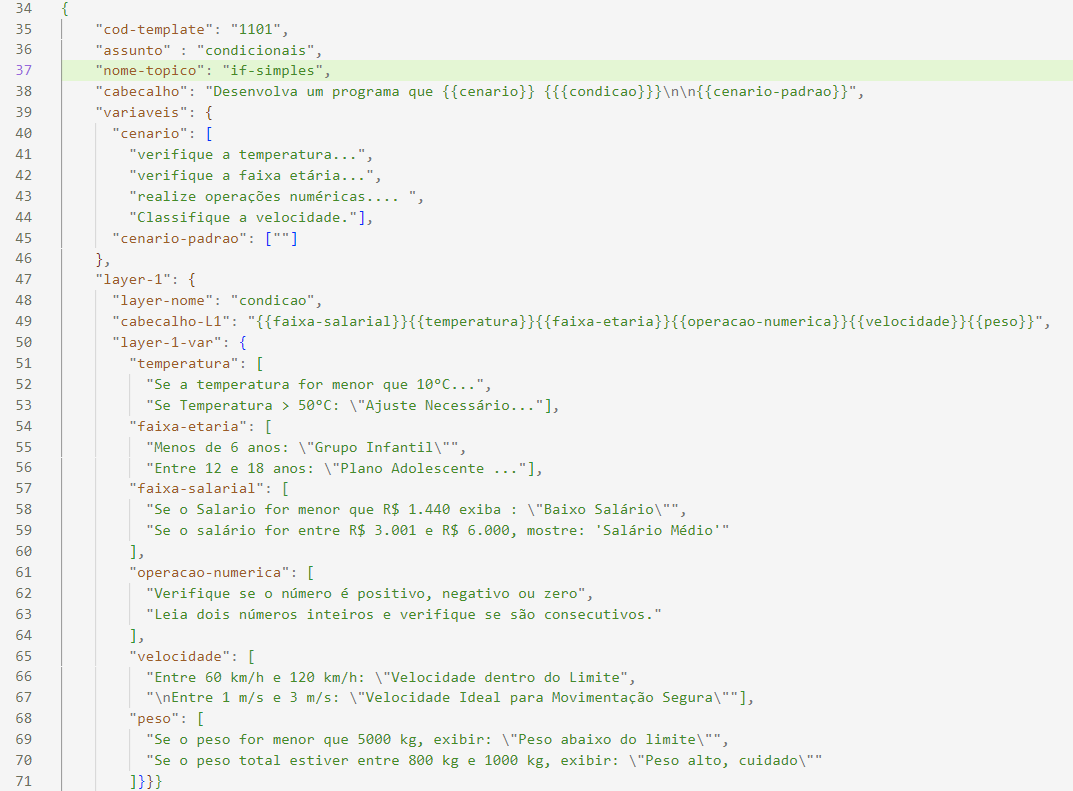
\includegraphics[width=16cm]{./imagens/capitulo7/json-de-template}
	\caption{JSON de Templates (Autoria Propria, 2025) }
	\label{fig:json-de-templates}
\end{figure}
\section{JSON de Questões}

O segundo componente é o JSON de Questões, ilustrado na \ref{fig:json-de-questoes}, cujo objetivo é definir o formato final de cada questão que será efetivamente apresentado aos estudantes. Neste arquivo, cada questão é identificado por um codigo, um titulo e um mapeamento de variáveis que aponta para as categorias estabelecidas no template. Assim essa estrutura não precisa carregar toda formatação do enunciado, mais apenas fazer referencias aos elementos já definidos no template. Assim, não é necessário carregar toda formatação do enunciado em cada questão, mas apenas fazer referencia aos elementos já definidos. Essa separação favorece a reutilização do mesmo modelo em diversas situações, bastando alterar os atributos de cada problema conforme necessário.

\begin{figure}[ht]
	\centering
	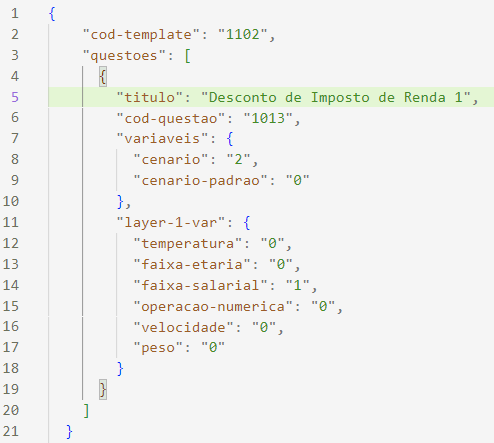
\includegraphics[width=14cm]{./imagens/capitulo7/json-de-questoes}
	\caption{JSON de Templates (Autoria Propria, 2025) }
	\label{fig:json-de-questoes}
\end{figure}
Na próxima seção serão discutidos os aspectos de implementação, mostrando como a geração de questões pode ser aplicada na prática e como os dados dos arquivos JSON são processados para gerar  as questões na prática.

\section{Ferramenta}

A ferramenta desenvolvida para a criação automatizada de questões de programação, este exemplo mostra estruturas condicionais “if” e “else”. O modelo proposto  tem como base um problema acompanhado de uma tabela de comparação, de modo que os estudantes possam escrever códigos para resolver diferentes cenários. Essa abordagem contribui para a compreensão do funcionamento das instruções condicionais ao permitir que o estudante teste, na prática, como as condições se comportam em diversos cenários. Além disso, o template adotado oferece a possibilidade de combinar múltiplos cenários em uma única tabela de comparação, bem como utilizar várias tabelas para um mesmo cenário, ampliando significativamente a quantidade de questões geradas. 

A flexibilidade desse template faz com que seja possível criar muitas variações de exercícios, cada um abordando aspectos distintos das estruturas condicionais. Ao selecionar o assunto e o tópico de interesse, uma questão é produzida dinamicamente, sendo exibida ao estudante juntamente com a tabela de comparação que auxilia na formulação do raciocínio. Em seguida, o código é escrito no ambiente de resolução proposto e submetido para avaliação. Para efetuar a correção, a ferramenta conta com o suporte de uma IA generativa, que verifica os casos de teste associados ao problema e fornece feedback imediato quanto ao desempenho. Essa estratégia incentiva o aprimoramento constante do aluno, pois o mesmo pode corrigir e reenviar sua solução até alcançar o resultado desejado 
\begin{figure}[ht]
	\centering
	\caption{Ferramenta (Autoria Propria, 2025) }
	\label{fig:ferramenta}
\end{figure}



Embora a configuração inicial dos templates exija um certo esforço de elaboração, esse investimento é compensado pela possibilidade de reutilizar as questões em diversas situações, reduzindo a necessidade de criar novos problemas para cada turma ou semestre. Uma vez que o repositório de problemas e cenários esteja consolidado, os docentes podem extrair diferentes conjuntos de exercícios de forma rápida, adequando-os a diferentes turmas, níveis de dificuldade ou contextos de aplicação. A prática frequente com casos variados também permite aos estudantes um aprendizado mais consistente, pois eles entram em contato com diversas nuances do uso das estruturas condicionais, refinando sua capacidade de resolução de problemas.

Na Figura 10, observa-se uma representação do repositório de questões, no qual a combinação entre o template e as tabelas de comparação ocorre de maneira automática, gerando problemas específicos a cada seleção realizada pelo estudante ou professor. Na Figura 12, está ilustrado o momento em que o aluno acessa o assunto escolhido, recebe a questão de forma dinâmica e submete seu código para correção. Esse processo evidencia como a ferramenta, ao integrar geração de conteúdo e avaliação automática, proporciona um ambiente de aprendizado ativo e personalizado. Dessa forma, a proposta oferece um caminho promissor para aprimorar o ensino de programação, otimizando tanto o trabalho do docente na elaboração de questões quanto o desenvolvimento das habilidades de resolução de problemas por parte dos estudantes.

 
